\documentclass{../exhibit}

\title{Battleship}

%% Font
\usepackage{imfellEnglish}
\usepackage[T1]{fontenc}
\raggedright

\usepackage{background}

\backgroundsetup{
scale=1,
color=black,
opacity=0.4,
angle=0,
contents={%
  \includegraphics[height=\paperheight]{mapBackground.jpg}%%https://upload.wikimedia.org/wikipedia/commons/8/81/Nautical_chart_of_the_West_Indies_1797.jpg
  }%
}




%% For the context
%% https://tex.stackexchange.com/questions/86150/torn-page-effect/86151#86151
\usepackage{tikz}
\usetikzlibrary{decorations.pathmorphing}
\definecolor{paper}{RGB}{239,227,157}





\renewcommand{\maketitle}{ %
  \begin{center}
    \scalebox{8}{\thetitle}
  \end{center}
  
\begin{tabular*}{\textwidth}{c @{\extracolsep{\fill}} c}  
\resizebox{4in}{!}{\begin{minipage}[b]{3in}\huge\directions\end{minipage}} &
  \resizebox{4in}{!}{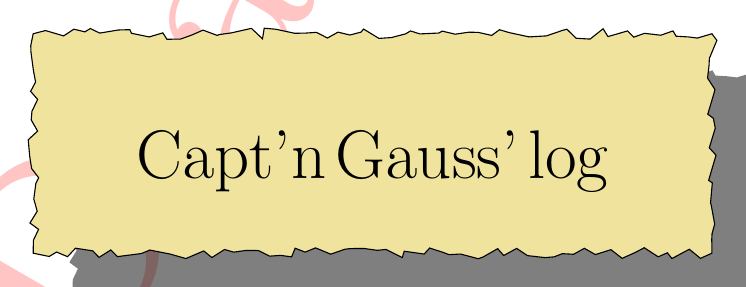
\begin{tikzpicture}[pencildraw/.style={ %
    decorate,
    decoration={random steps,segment length=4pt,amplitude=2pt}
    } %
]
\node[
preaction={fill=black,opacity=.5,transform canvas={xshift=.5cm,yshift=-.5cm}},
pencildraw,draw,fill=paper,text width=3in,inner sep=.5cm] 
{\begin{center}\Huge Capt'n Gauss' log \end{center}\vspace{.7cm} {\huge\context}};
\end{tikzpicture}}

\end{tabular*}

\vfill

\includegraphics[width=3in]{logoPirate.png}\hfill \includegraphics[width=2in]{bammLogo.png}


}


\begin{document}

\begin{context}
  With this here coordinate system, we will use our minds to outwit
  our opponents.
  \\[1cm]
    Batten down the hatches, time to sink some ships!

  
\end{context}

\begin{directions}
\begin{itemize}
\item First, you secretly put your ships on the grid.
\item Then, you take turns guessing where your friend's ships are. If
  you guess right, your friend marks the ``hit'' and you get to guess
  again.  If you guess wrong, it's your friend's turn.
\item The game goes on until one of you sinks all of the other person's
ships.
\end{itemize}

\end{directions}

\begin{example}%%https://commons.wikimedia.org/wiki/File:Battleship_game_board.svg
    \begin{center}
    \includegraphics[width=.5\textwidth]{gameboard.png}
  \end{center}
\end{example}

\begin{mathConnections}
  https://bartsnapp.github.io/Math-Outreach-Exhibits/battleship/
\end{mathConnections}

\end{document}
